\documentclass[a4paper, 12pt]{article}
\usepackage{graphicx}
\usepackage{amssymb, amsfonts, amsmath, amsthm}
\usepackage[margin=1in]{geometry}
\usepackage{enumitem}
\usepackage{array}
\usepackage{fancyhdr}
\usepackage{tikz}
\usepackage{parskip}
\usepackage{float}
\usetikzlibrary{automata, positioning, arrows}

\setlength{\headheight}{14.49998pt}

\tikzset {
    ->,
    >=stealth',
    node distance=3cm,
    every state/.style={thick, fill=gray!10},
    initial text = $ $
}

\makeatletter
\renewenvironment{proof}[1][\proofname]{\par
%  \pushQED{\qed}% <--- remove the QED business
  \normalfont \topsep6\p@\@plus6\p@\relax
  \trivlist
  \item[\hskip\labelsep
        \itshape
    #1\@addpunct{.}]\ignorespaces
}{%
%  \popQED% <--- remove the QED business
  \endtrivlist\@endpefalse
}
\renewcommand\qedhere{} % to ensure code portability
\makeatother

\pagestyle{fancy}
\fancyhead[l]{SECJ3203}
\fancyhead[c]{Tutorial 3}
\fancyhead[r]{19 April 2024}

\title{Tutorial 3 & 4}
\date{}
\author{}

\renewcommand{\proofname}{Solution:}

\begin{document}
    \begin{enumerate}
        \item
        \begin{enumerate}
            \item M1: \( \{q_0\}\) M2: \(\{q_0\}\)
            \item M1: \(\{q_1\}\) M2: \( \{q_0, q_3\} \)
            \item M1: 
            $\begin{aligned}[t]
                [q_0, aabb] &\vdash [q_1, abb] \\
                &\vdash [q_2, bb] \\
                &\vdash [q_0, b] \\
                &\vdash [q_0, \lambda]
            \end{aligned}$ 
            \vspace{5pt} \newline
            Sequence of states: $q_0 \to q_1 \to q_2 \to q_0 \to q_0$  
            
            M2:
            $\begin{aligned}[t]
                [q_0, aabb] &\vdash [q_0, abb] \\
                &\vdash [q_0, bb] \\
                &\vdash [q_1, b] \\
                &\vdash [q_3, \lambda]
            \end{aligned}$ \hfill
            \vspace{5pt} \newline
            Sequence of states: $q_0 \to q_0 \to q_0 \to q_1 \to q_3$
            \item M1 does not accept the string \(aabb\) but M2 does.
            \item M1 does not accept \(\varepsilon\) but M2 does.
            \item M1 \(= (\{q_0, q_1, q_2\}, \{a, b\}, \delta, q_0, q_1)\) where \(\delta\) is described as: 
            \begin{center}
                
            \begin{tabular}{c|cc}
                 & $a$ & $b$ \\ \hline
            $q_0$ & $q_1$ & $q_0$ \\ 
            $q_1$ & $q_2$ & $q_2$ \\ 
            $q_2$ & $q_1$ & $q_0$
            \end{tabular}

            \end{center}
            \vspace{5mm}

            M2 \(= (\{q_0, q_1, q_2, q_3\}), \{a, b\}, \delta, q_0, \{q_0, q_3\})\) where \(\delta\) is described as:
            \begin{center}

            \begin{tabular}{c|cc}
                 & $a$ & $b$ \\ \hline
                $q_0$ & $q_0$ & $q_1$ \\
                $q_1$ & $q_2$ & $q_3$ \\
                $q_2$ & $q_1$ & $q_0$ \\
                $q_3$ & $q_2$ & $q_3$
            \end{tabular}
            \end{center}
        \end{enumerate}
        \item
        \begin{enumerate}
            \item \makebox[0pt][r]{\quad}

            \begin{minipage}{\linewidth}
                \centering
                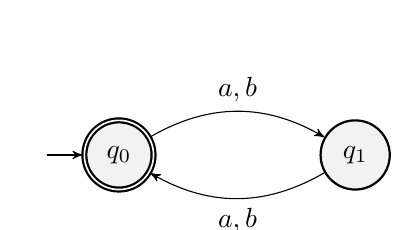
\begin{tikzpicture}
                    \node[state, initial, accepting] (q0) {$q_0$};
                    \node[state, right of=q0] (q1) {$q_1$};

                    \draw 
                    (q0) edge[bend left, above] node{$a, b$} (q1)
                    (q1) edge[bend left, below] node{$a, b$} (q0);
                    \end{tikzpicture}
            \end{minipage}
            
            \item 
            \textbf{\textit{abbb}}:
            \( \begin{aligned}[t]
                [q_0, abbb] &\vdash [q_1, bbb] \\
                &\vdash [q_0, bb] \\
                &\vdash [q_1, b] \\
                &\vdash [q_0, \lambda]
            \end{aligned} \)

            All alphabets are traced and the machine stops at $q_0$, which is an accepting state. Thus, this machine accepts the string $abbb$.

            \textbf{\textit{bbb}}:
            \( \begin{aligned}[t]
                [q_0, bbb] &\vdash [q_1, bb] \\
                &\vdash [q_0, b] \\
                &\vdash [q_1, \lambda]
            \end{aligned} \)

            All alphabets are traced and the machine stops at $q_1$, which is not an accepting state. Thus, this machine rejects the string $bbb$.

            \textbf{\textit{baa}}:
            \( \begin{aligned}[t]
                [q_0, baa] &\vdash [q_1, aa] \\
                &\vdash [q_0, a] \\
                &\vdash [q_1, \lambda]
            \end{aligned} \)

            All alphabets are traced and the machine stops at $q_1$, which is not an accepting state. Thus, this machine rejects the string $baa$.

            \textbf{\textit{baab}}:
            \( \begin{aligned}[t]
                [q_0, baab] &\vdash [q_1, aab] \\
                &\vdash [q_0, ab] \\
                &\vdash [q_1, b] \\
                &\vdash [q_0, \lambda]
            \end{aligned} \)

            All alphabets are traced and the machine stops at $q_0$, which is an accepting state. Thus, this machine accepts the string $baab$.

            \item The strings $abbb$ and $baab$ are accepted by the machine $M$.
            \item $((a+b)(a+b))^*$
        \end{enumerate}
    \end{enumerate}

    \newpage
    \fancyhead[c]{Tutorial 4}

    \begin{enumerate}
        \item
        \begin{enumerate}
            \item 
            \begin{tabular}{c|cc}
                 & $a$ & $b$  \\ \hline
             $q_0$ & $q_1$ & $q_0$ \\
             $q_1$ & $q_2$ & $q_0$ \\
             $q_2$ & $q_3$ & $q_0$ \\
             $q_3$ & $q_3$ & $q_3$
            \end{tabular}
            
            $M$ is a deterministic FA.
            \item
            \textbf{\textit{aaa}}: \( \begin{aligned}[t]
                [q_0, aaa] &\vdash [q_1, aa] \\
                &\vdash [q_2, a] \\
                &\vdash [q_3, \lambda]
            \end{aligned} \)

            All alphabets are traced and the machine stops at $q_3$, which is an accepting state. Thus, this machine accepts the string $aaa$.

            \textbf{\textit{aab}}: \( \begin{aligned}[t]
                [q_0, aab] &\vdash [q_1, ab] \\
                &\vdash [q_2, b] \\
                &\vdash [q_0, \lambda]
            \end{aligned} \)

            All alphabets are traced and the machine stops at $q_0$, which is not an accepting state. Thus, this machine rejects the string $aab$.

            \textbf{\textit{baaab}}: \( \begin{aligned}[t]
                [q_0, baaab] &\vdash [q_0, aaab] \\
                &\vdash [q_1, aab] \\
                &\vdash [q_2, ab] \\
                &\vdash [q_3, b] \\
                &\vdash [q_3, \lambda]
            \end{aligned} \)

            All alphabets are traced and the machine stops at $q_3$, which is an accepting state. Thus, this machine rejects the string $baaab$.

            \item The strings $aaa$ and $baaab$ are accepted by $M$.
            \item $(a+b)^*aaa(a+b)^*$
        \end{enumerate}

        \item
        \begin{enumerate}
            \item 
            $L_1 = (a+b)^*$ 
        
            \begin{minipage}{\linewidth}
                \centering
                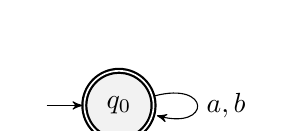
\begin{tikzpicture}
                    \node[state, initial, accepting] (q0) {$q_0$};

                    \draw 
                    (q0) edge[loop right] node{$a, b$} (q0);
                    \end{tikzpicture}
            \end{minipage}

            \item
            $L_2 = (a+b)(a+b)^*$

            \begin{minipage}{\linewidth}
                \centering
                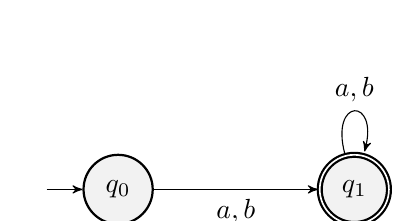
\begin{tikzpicture}
                    \node[state, initial] (q0) {$q_0$};
                    \node[state, accepting, right of=q0] (q1) {$q_1$};

                    \draw 
                    (q0) edge[below] node{$a, b$} (q1)
                    (q1) edge[loop above] node{$a, b$} (q1);
                    \end{tikzpicture}
            \end{minipage}
            \vfill

            \item 
            $L_3 = ba(a+b)^*$

            \begin{minipage}{\linewidth}
                \centering
                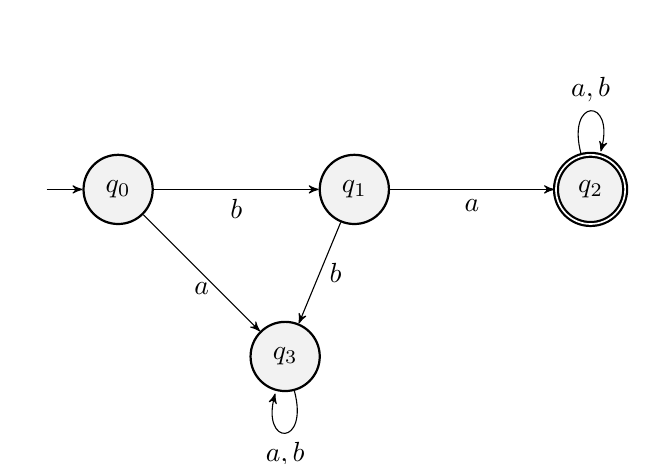
\begin{tikzpicture}
                    \node[state, initial] (q0) {$q_0$};
                    \node[state, right of=q0] (q1) {$q_1$};
                    \node[state, accepting, right of=q1] (q2) {$q_2$};
                    \node[state, below right of=q0] (q3) {$q_3$};

                    \draw 
                    (q0) edge[below] node{$b$} (q1)
                    (q1) edge[below] node{$a$} (q2)
                    (q0) edge[below] node{$a$} (q3)
                    (q1) edge[below, right = 0.3] node{$b$} (q3)
                    (q2) edge[loop above] node{$a, b$} (q2)
                    (q3) edge[loop below] node{$a, b$} (q3);
                    \end{tikzpicture}
            \end{minipage}

            \item 
            $L_4=(a+b)^*ba$

            \begin{minipage}{\linewidth}
                \centering
                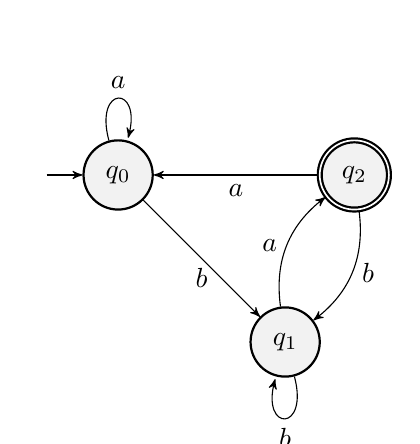
\begin{tikzpicture}
                    \node[state, initial] (q0) {$q_0$};
                    \node[state, below right of=q0] (q1) {$q_1$};
                    \node[state, accepting, right of=q0] (q2) {$q_2$};

                    \draw 
                    (q0) edge[loop above] node{$a$} (q0)
                    (q0) edge[below] node{$b$} (q1)
                    (q1) edge[loop below] node{$b$} (q1)
                    (q1) edge[bend left] node[left=0]{$a$} (q2)
                    (q2) edge[bend left] node[right]{$b$} (q1)
                    (q2) edge[below] node{$a$} (q0);
                    \end{tikzpicture}
            \end{minipage}

            \item $L_5=ba((a+b)^*ba+\lambda)$
        \end{enumerate}
    \end{enumerate}
    
\end{document}
